\section{Prerequisities}
\label{sec:prerequisities}

% \subsection{Basics of the \glsfmtlong{fem}}

The basic idea of the \glsfmtlong{fem} conforms to the specification of a function space and finding a solution to the investigated problem in it. To be more precise, we pick a suitable set of basis functions for which the solution is a linear combination. Its coefficients are called unknowns or \glspl{dof}, since their values are determined after solving the problem.

In general, \gls{fem} requires a subdivision of the domain $\Omega$ into smaller cells $K$, where $\Omega = \cup_{i} K_i$ and each cell $K$ corresponds to a connected Lipschitz domain with nonempty interior \todo{Check Ciarlet definition?}. Typical choices for cells are triangles or quadrilaterals in two and tetrahedra or hexahedra in three dimensions.
%All these cells are mappings of a reference cell, to which we assign a set of shape functions with corresponding support points.
%Those functions are designed to have the value one on exactly one support point and the value zero on all others.
Further, on each cell $K$, we define a finite-dimensional function space $P$, accompanied by a set of functionals $N = {\Psi_1, \dots, \Psi_n}$ that are a basis to its dual space $P'$, where $n$ corresponds the number of nodes. The tuple $(K,P,N)$ is called a finite element. \todo{Cite Ciarlet or Brenner. Depends on definition of K.}

With this definition, we are able to find a set of basis functions ${\varphi_1, \dots, \varphi_n}$ of $P$ dual to $N$ fulfilling $\Psi_i(\varphi_j) = \delta_{ij}$. In other words, these basis functions span the function space $P$ while each of them has the value one on their associated node and zero on the other. They form our finite element approximation as a linear combination $u_{\text{hp}}(\vec{x}) = \sum_{j} U_j \, \varphi_j(\vec{x})$, where coefficients $U_j$ are known as \glsfmtlongpl{dof}.

We transform the original problem into a variation one by converting it to a weak formulation. This process belongs to the class of Galerkin methods, of which we distinguish between \gls{cg} and \gls{dg} methods. For the former, we require that our finite element approximation is continuous across cell interfaces resulting in shared \glspl{dof} on all transitions. For discontinuous methods, jumps of the approximation are possible on cell interfaces, and thus each cell has its own set of \glspl{dof} from which none are shared. Here, relations between cells are quantified via penalty methods that correlate \glspl{dof} on interfaces of neighboring cells.

With the weak formulation of the investigated problem, we are left to assemble and solve the corresponding system of linear equations for the unknown coefficients or \glspl{dof}. In practice, we calculate the corresponding integrals using quadrature rules and basis functions which have been mapped from a reference cell $\widehat{K}$.

When dealing with finite elements in practice, it is sufficient to work with nodes and shape functions once the type of element is specified. One of the most common types of finite elements are Lagrangian elements, that are based on Lagrangian interpolation. The distribution of nodes on quadrilaterals in Lagrangian elements up to fourth order polynomials are depicted in Fig.~\ref{fig:lagrange}.

\begin{figure}
\begin{subfigure}{.24\textwidth}
  \centering
  \input{figures/parallel/q1}
  \caption{$Q_1$ element.}
\end{subfigure}
\begin{subfigure}{.24\textwidth}
  \centering
  \input{figures/parallel/q2}
  \caption{$Q_2$ element.}
\end{subfigure}
\begin{subfigure}{.24\textwidth}
  \centering
  \begin{tikzpicture}[scale=2]
\def\Length{1}
\def\Radius{0.03}

\LagrangeCell{0}{0}{\Length}{\Radius}{3}
{{,,,,,,,,,,,,,,,}};
\end{tikzpicture}
  \caption{$Q_3$ element.}
\end{subfigure}
\begin{subfigure}{.24\textwidth}
  \centering
  \begin{tikzpicture}[scale=2]
\def\Length{1}
\def\Radius{0.03}

\LagrangeCell{0}{0}{\Length}{\Radius}{4}
{{,,,,,,,,,,,,,,,,,,,,,,,,}};
\end{tikzpicture}
  \caption{$Q_4$ element.}
\end{subfigure}
\caption[Lagrangian elements $Q_p$.]{First four Lagrangian elements $Q_p$ on quadrilateral unit cells with $(1+p)^\text{dim}$ nodes each.}
\label{fig:lagrange}
\end{figure}

This is just a brief introduction to \gls{fem} in order to provide the fundamentals for this chapter and to specify the nomenclature used. More details on this topic can be found in common literature \parencite[e.g.][]{girault1986, elman2014, kuzmin2015} \todo{add more literature?}. Especially \textcite{brenner2008} provided a more rigorous and mathematically sound definition on finite elements.


\subsection{Adaptive methods for \glsfmtshort{fem}}

In computational applications, adaptive methods are used to align the resolution or rather the processing power to the complexity of the investigated problem, i.e.\@ to specific sections of the domain. In terms of grid refinement, cells will be split twice per dimension, resulting in two, four or eight children in one, two or three dimensions, respectively. On the contrary, we join the corresponding amount of cells to their parent cell for grid coarsening. This process is also known as \h-adaptation, referring to adjusting the cell's length or diameter \(h\) locally. We require hierarchic relations between parent cells and their children that motivate the use of tree structures rooting in each cell of the initial coarse mesh. Combined this leads to a forest structure, in which each level corresponds to a full representation of the domain. The entirety of all leaves in this forest resembles the computational domain relevant for assembling and solving the system of equations. These particular cells, which have no children, are called active cells and are the only ones carrying \glspl{dof}. For more information, \textcite{bangerth2003} have elaborated more rigorously on grid adaptation, especially for the \gls{fem} method.

As an alternative to modifying the grid resolution, we can also adapt the function space using various finite elements associated with each cell. These finite elements may differ in the polynomial degree $p$ of their shape functions, offering the unique possibility for \p-adaptation, or \hp-adaptation when used together with grid adaptation.

Refinement level differences on quadrilateral or hexahedral meshes, as well as varying finite elements on neighboring active cells lead to hanging nodes which are nodes with no counterpart on the opposite side of the interface. In combination with \gls{cg} methods, the finite element approximation needs to be continuous on these nodes as well, which requires  constraining them to the surrounding ones. A depiction of \h- and \p-adaptive domains along with hanging nodes is presented in Fig.~\ref{fig:hpadaptivity}.

\begin{figure}
\begin{subfigure}{0.49\textwidth}
  \centering
  \begin{tikzpicture}[scale=2]
\def\Length{0.5}
\def\Radius{0.03}

\LagrangeCell{-2*\Length}{0}{2*\Length}{\Radius}{2}
{{,,,,,,,,}};

\LagrangeCell{0}{0}{\Length}{\Radius}{2}
{{,,,,,,,,}};
\LagrangeCell{\Length}{0}{\Length}{\Radius}{2}
{{,,,,,,,,}};
\LagrangeCell{0}{\Length}{\Length}{\Radius}{2}
{{,,,,,,,,}};
\LagrangeCell{\Length}{\Length}{\Length}{\Radius}{2}
{{,,,,,,,,}};
\end{tikzpicture}
  \caption{\h-adaptation.}
\end{subfigure}
\begin{subfigure}{0.49\textwidth}
  \centering
  \input{figures/parallel/padaptivity}
  \caption{\p-adaptation.}
\end{subfigure}
\caption{Example of an \h-adapted mesh consisting of quadrilateral cells. Differences in the refinement level of neighboring cells gives rise to hanging nodes.}
\label{fig:hpadaptivity}
\end{figure}

For convenience, the level difference of neighboring cells is usually limited to one level in order to simplify interpolation between cell interfaces. For quadrilateral or hexahedral meshes, this \textit{2:1 mesh balance} ensures to limit the occurrence of hanging nodes.

Adaptive methods in the finite element context have been elaborated by \textcites{bangerth2003}{bangerth2009}.

% make this part of the next chapter?
%When the function space is a subset of a different finite element, we say that it dominates the other finite element.

%Dominating finite elements own \glspl{dof} on cell interfaces, with some minor exceptions as elaborated by \textcite{bangerth2009} who also provide more information on \hp-refinement.




\subsection{Parallelization of \glsfmtshort{fem}}

\Gls{hpc} applications requires scalable algorithms and data structures for machines with distributed memory, which we realize using the \gls{mpi} standard. In this context, the workload on all participating processes will be shared by partitioning the whole domain among them.

These ambitions pose different challenges on the design of data structures and information exchange between processes. Especially dynamic changes of the domain by \hp-adaptation are difficult, since they require the redistribution of the workload by repartitioning the global mesh, as well as the transfer of data not only between processes, but also between the former and the updated mesh. Here, we distinguish between different subsets of cells and \glspl{dof} which will be introduced in the following.

Each process will only store data of cells that belong to its owned section of the domain. Those cells are called \textit{locally owned cells}, and all \glspl{dof} on them are referred to as \textit{locally active \glspl{dof}}. Every \gls{dof} will be uniquely enumerated on the global mesh. With \gls{cg} methods, \glspl{dof} on interfaces between cells of different processes may be owned by either one or the other. Thus, not all \glspl{dof} on locally owned cells have to be \textit{locally owned \glspl{dof}}.

During the assembly of equation systems, we need to refer to surrounding cells that do not belong to the local domain. Typically, the halo spanning one level of cells around the locally owned domain is sufficient. We call these cells \textit{ghost cells}. Data from ghost cells has to be requested from the owning process. The combination of locally owned and ghost cells and their corresponding \glspl{dof} are labeled \textit{locally relevant}.

Further, we require that every process stores a copy of the common coarse mesh. This allows an easy construction of the whole grid during repartitioning just with adaptive methods. We establish the 2:1 mesh balance on all cells of the local mesh, leaving refined cells that are not actually used. These cells that are not locally relevant will be called \textit{artificial cells}. An example of a distributed, adapted mesh is shown in Fig.~\ref{fig:paralleldistribution} with all presented classes of cells.

\begin{figure}
\begin{subfigure}{.49\textwidth}
  \centering
  \input{figures/parallel/distribution_rank0}
  \caption{Process with rank 0.}
\end{subfigure}
\begin{subfigure}{.49\textwidth}
  \centering
  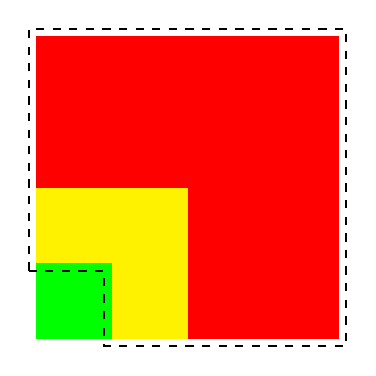
\begin{tikzpicture}[scale=0.96]
\def\Length{1}
\def\Radius{0.06}

% mark types of cells
\fill[color=red] (0,2*\Length) rectangle (4*\Length,4*\Length);
\fill[color=red] (2*\Length,0) rectangle (4*\Length,2*\Length);
\fill[color=yellow] (0,\Length) rectangle (2*\Length,2*\Length);
\fill[color=yellow] (\Length,0) rectangle (2*\Length,\Length);
\fill[color=green] (0,0) rectangle (\Length,\Length);

% plot mesh
\def\XPos{0}
\def\YPos{0}
\LagrangeCell{\XPos}{\YPos}{\Length}{\Radius}{1}{{,,,}};
\LagrangeCell{\XPos}{\YPos+\Length}{\Length}{\Radius}{1}{{,,,}};
\LagrangeCell{\XPos+\Length}{\YPos}{\Length}{\Radius}{1}{{,,,}};
\LagrangeCell{\XPos+\Length}{\YPos+\Length}{\Length}{\Radius}{1}{{,,,}};

\def\XPos{2*\Length}
\def\YPos{0}
\LagrangeCell{\XPos}{\YPos}{\Length}{\Radius}{1}{{,,,}};
\LagrangeCell{\XPos}{\YPos+\Length}{\Length}{\Radius}{1}{{,,,}};
\LagrangeCell{\XPos+\Length}{\YPos}{\Length}{\Radius}{1}{{,,,}};
\LagrangeCell{\XPos+\Length}{\YPos+\Length}{\Length}{\Radius}{1}{{,,,}};

\LagrangeCell{0}{2*\Length}{2*\Length}{\Radius}{1}{{,,,}};
\LagrangeCell{2*\Length}{2*\Length}{2*\Length}{\Radius}{1}{{,,,}};

% frame relevant cells
\def\Offset{0.1}
\draw[dashed, thick] (-\Offset,\Length-\Offset) -- (-\Offset,4*\Length+\Offset) -- (4*\Length+\Offset,4*\Length+\Offset) -- (4*\Length+\Offset,-\Offset) -- (\Length-\Offset,-\Offset) -- (\Length-\Offset,\Length-\Offset) -- cycle;
\end{tikzpicture}
  \caption{Process with rank 1.}
\end{subfigure}
\caption{Parallel distribution of an \h-adapted mesh on two processes.}
\label{fig:paralleldistribution}
\end{figure}

%This is just a brief outline of all the requirements that \textcite{bangerth2012} worked out, which is crucial for the upcoming section.

%We work with \dealii{}. This library works with quadrilaterals and hexahedrals only. All the considerations in this dissertation should be easily applicable on triangles and tetrahedra as well.

%In the \dealii{}, the parallel is handed out to an oracle that is requested on all mesh related operations. \dealii{} offers an interface to the \pforest{} library.

\textcite{bangerth2012} worked out the parallelization of \h-adaptive \gls{fem} within the \dealii{} library in great detail.